\section{Implementation and Evaluation} \label{sec:imp&eva}

In the previous sections, we presented the RADIUS system design and analyzed the impact of its parameters on the detection performance. Based on these, we implemented the DA component of RADIUS for TelosB sensor platforms and the VCC for standard PCs. In this section, we detail our implementation and discuss the system overhead. At last, we show the evaluation results on the detection performance of the overall implemented system in an indoor testbed. 

\subsection{System Implementation} 

In this section, we first describe the implementation details of the two major RADIUS components: the DA and the VCC. We introduce the programming interface of the DA to show that it is easy to use for higher-layer services and applications, followed by the implementation details of the VCC and of the RADIUS IoT extension. 
%Then, we evaluate the implementation overhead to show that it is lightweight enough to be executed on actual sensor nodes. 

\begin{figure}[h]
	\vspace{-0.3cm}
	\begin{lstlisting}[frame=single]  % Start your code-block
	
	interface DetectionAgent {
	command void configureDA(Struct_Param parameters);
	command error_t start_Training();
	command error_t stop_Training();
	command error_t start_Detection();
	command error_t stop_Detection();
	command void update_RSSI(uint8_t rssi, uint8_t childId);
	}
	\end{lstlisting}
	\vspace{-0.55cm}
	\caption{\textbf{The programming interface for DA.}}
	\label{fig:TinyOSinterface}
	\vspace{-0.3cm}
\end{figure}



To ease the integration of RADIUS into higher-layer applications, we implemented the DA component as a module on TinyOS 2.1.2, which provides an interface \texttt{DetectionAgent} (see Figure \ref{fig:TinyOSinterface}). The \texttt{configureDA} command is used to configure DA with user-specified parameter settings (e.g., the initial $P(H_g)$) as provided in configuration messages sent by the VCC. The interface also provides control commands such as \texttt{start\_Training} or \texttt{start\_Detection} for executing the different phases in RADIUS. The command \texttt{update\_RSSI} is used to update the RSSI distribution of each link during both the training and the detection phases. With this programming interface, an application only needs to react to VCC's control messages and call the different commands accordingly. Note that RADIUS is not restricted to TelosB or TinyOS and can be easily adapted to other embedded devices with low-power radios.
% without the need to handle all specific details in RADIUS. 



\begin{figure}[t]
	%\vspace{-0.2cm}
	\centering
	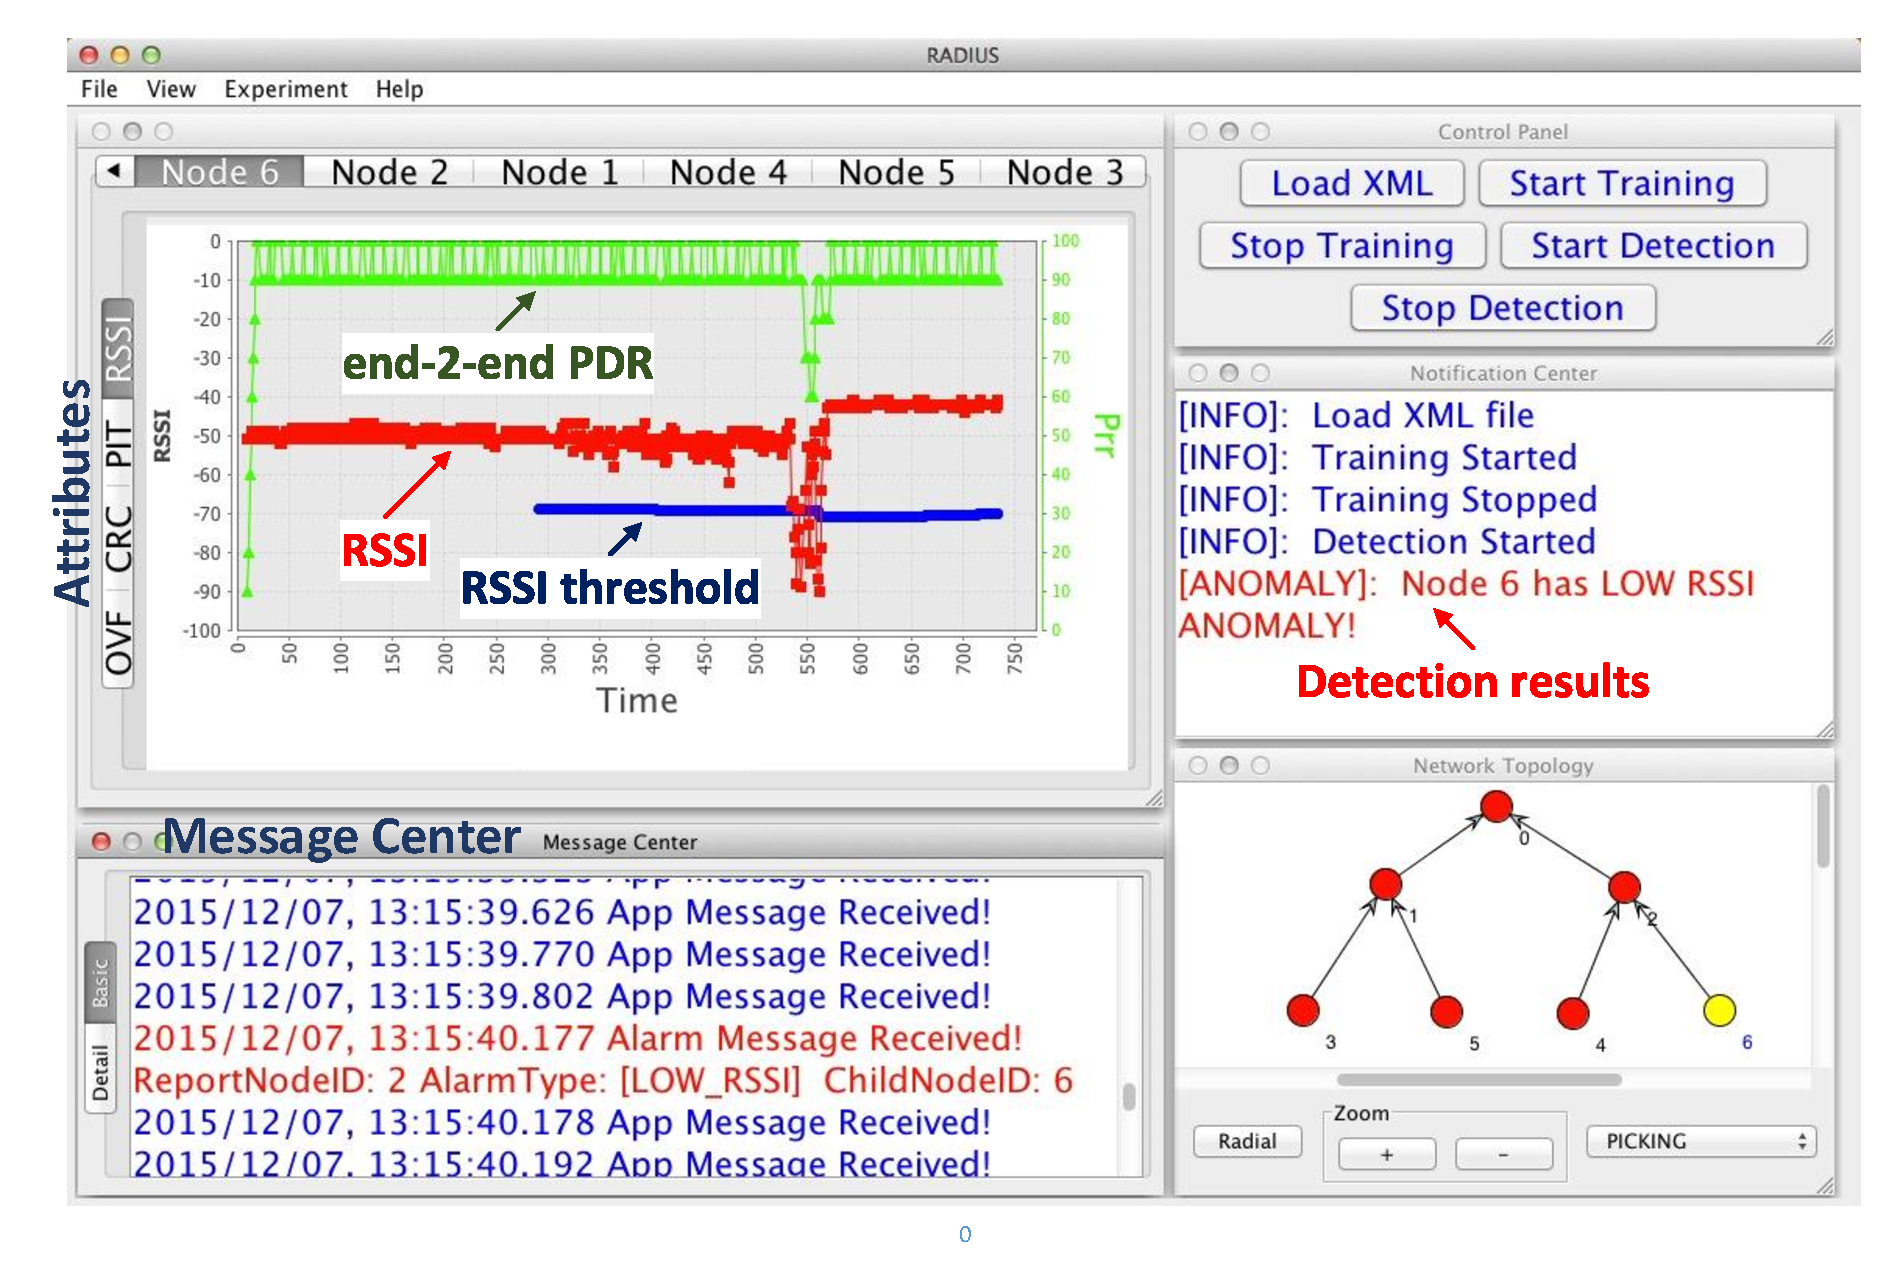
\includegraphics[width=1\linewidth, height = 5.5cm]{Radius-GUI}
	\vspace{-0.9cm}
	\caption{\textbf{The Monitoring User Interface of VCC.}}
	\label{fig:GUI}
	\vspace{-0.7cm}
\end{figure}


\begin{figure}[t]
	%\vspace{-0.3cm}
	\centering
	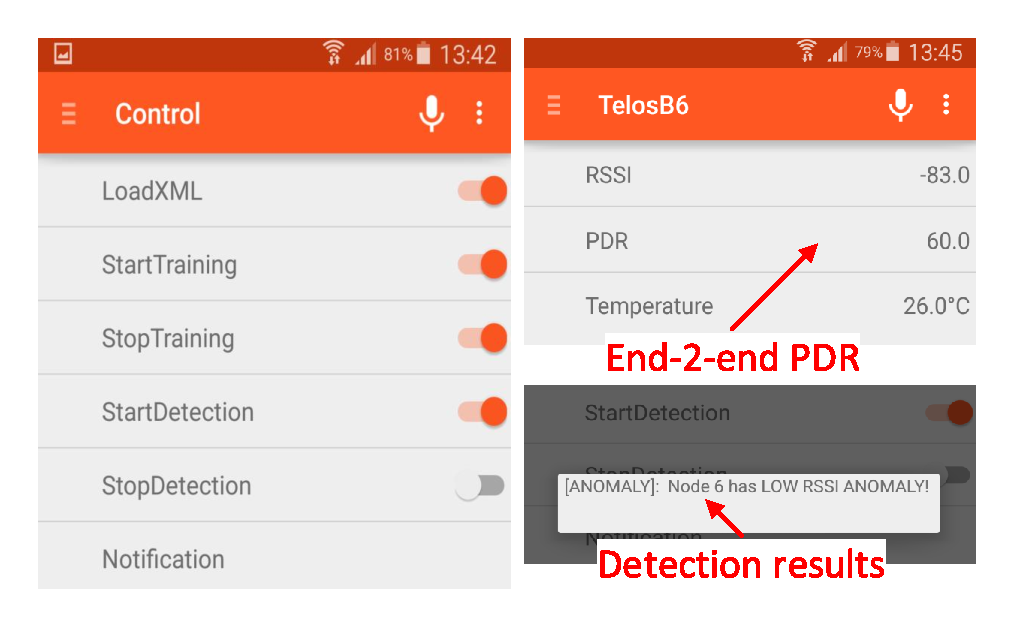
\includegraphics[width=1\linewidth, height = 5.5cm]{IOT-interface}
	\vspace{-0.9cm}
	\caption{\textbf{The Android UI for RADIUS.}}
	\label{fig:IOT}
	\vspace{-0.7cm}
\end{figure}

The component VCC, running on a standard PC, is implemented in Java. It processes the alarms received from the network and produces diagnosis results reporting the relevant anomalies and their locations for the nodes that are experiencing high packet losses, which assists the system operator in identifying possible remedy actions. The VCC also includes a \textit{ Monitoring User Interface} (see Figure \ref{fig:GUI}), which provides a visualization of the packet delivery performance, detection status and the diagnosis results. Via this interface, the operator can monitor and control the RADIUS system.



We have also extended the VCC with an Internet-of-Things interface, which allows the VCC to connect with openHAB \cite{openHAB}, an open source smart home automation software. MQTT \cite{MQTT}, a lightweight messaging transport protocol, is used for the communication between openHAB and the VCC. With this extension, the user can remotely control the RADIUS system and monitor the detection results with an Android smart phone, as depicted in Figure \ref{fig:IOT}.



The current implementation of RADIUS is able to detect anomalies in link quality. Nevertheless, the programming interface (Figure \ref{fig:TinyOSinterface}) and the DA module can be easily extended to detect anomalies of other attributes, e.g., CRC error rate or packet overflow rate.
%, due to the modular implementation of the DA component. 
In addition, RADIUS currently works for static tree-based data collection applications but it can be also applied to other routing schemes. 
%E.g., before a node switches its parent, it informs the current parent node to stop monitoring for this node; after parent switch, the new parent node initiates a training phase. Once the thresholds are computed, it is ready to start the anomaly detection for this newly joined child node.




\subsection{System Overheads} \label{sec:overhead}
In this section, we analyze the memory, communication and computation overheads of our RADIUS implementation.

%\paragraph{Memory overhead.}

\paragraph{Memory overhead.} Detection Agents incur memory overhead on RAM (data) and ROM (program) of sensor nodes. As presented in Section \ref{sec:trainingSetUpdate}, we keep updating the training set to adapt the mean $\mu$ and standard deviation $\sigma$ of the density distribution of RSSI. To avoid increasing RAM usage during the update, we implemented this in a memory-friendly way, i.e., to compute $\mu$ and $\sigma$ with a single pass without storing the previous measurements of RSSI. To do so, we reformulate $\mu$  and $\sigma$ in the following way:
\setlength{\belowdisplayskip}{2pt} \setlength{\belowdisplayshortskip}{2pt}
\setlength{\abovedisplayskip}{2pt} \setlength{\abovedisplayshortskip}{2pt}
\begin{equation} \label{equ:stdComputation}
\mu = \frac{s}{n},   \quad  \sigma = \sqrt{\frac{1}{n-1}\big(q - \frac{s^2}{n}\big)}
\end{equation}
where $s$ and $q$ are defined as follows:
\begin{align}
s= \displaystyle \sum_i^n{x_i},\quad  q = \displaystyle \sum_i^n{x_i^2}
\end{align}
%\vspace{-0.1cm}
in which $x_i$ is the i-th RSSI reading. Instead of storing the entire training set, the DA then stores only 2 counters ($s$ and $q$) for each link to compute and update $\mu$ and $\sigma$. By doing so, the RAM consumption of RADIUS has a complexity of $O(mn)$, where $m$ is the number of links from direct child nodes and $n$ is the number of monitored attributes (e.g., RSSI, CRC error rate), remaining independent from the sample number.

To evaluate the RAM and ROM overhead, we compare the memory usage of a tree-based data collection application with and without the DA module. In the application, each node has two one-hop child nodes and therefore stores information about two links. The application alone consumes 3060 bytes in RAM and 25082 bytes in ROM while the application including the DA module consumes 3176 bytes in RAM and 31170 bytes in ROM. This indicates that the DA module consumes 116 bytes RAM (in comparison to 10 KB RAM in a TelosB device), and approximately 6 KB ROM (in comparison to 48 KB ROM in a TelosB device). %Such RAM overhead is small compared to 10 KB RAM in TelosB and the ROM overhead is acceptable compared to 48 KB ROM in TelosB. 

\paragraph{Communication overhead.} Due to its distributed architecture, the anomaly detection process alone incurs no communication overhead in RADIUS. It requires additional communication only if the DAs send alarms corresponding to detected anomalies, or when the VCC sends control messages. To reduce such overhead, the alarms with minimum information (2 bytes) about the detected anomaly are piggybacked on the application packets. On the other hand, the number of control messages delivered from the VCC to the DAs, based on our indoor testbed evaluation results, is negligible compared to the amount of received application packets.

\paragraph{Computation overhead.} The main computation overhead comes from the processing of the Bayesian thresholding. In RADIUS, the complexity of Bayesian thresholding involves the calculation of the mean, the standard deviation and the Bayes threshold according to Equation \ref{equ:rssiTHD}. Testing results show that the processing of a Bayes threshold takes about 10 ms, which is small compared to the normal packet inter-arrival time in typical data collection applications.


\begin{figure}[t]
	%\vspace{-0.4cm}
	\centering
	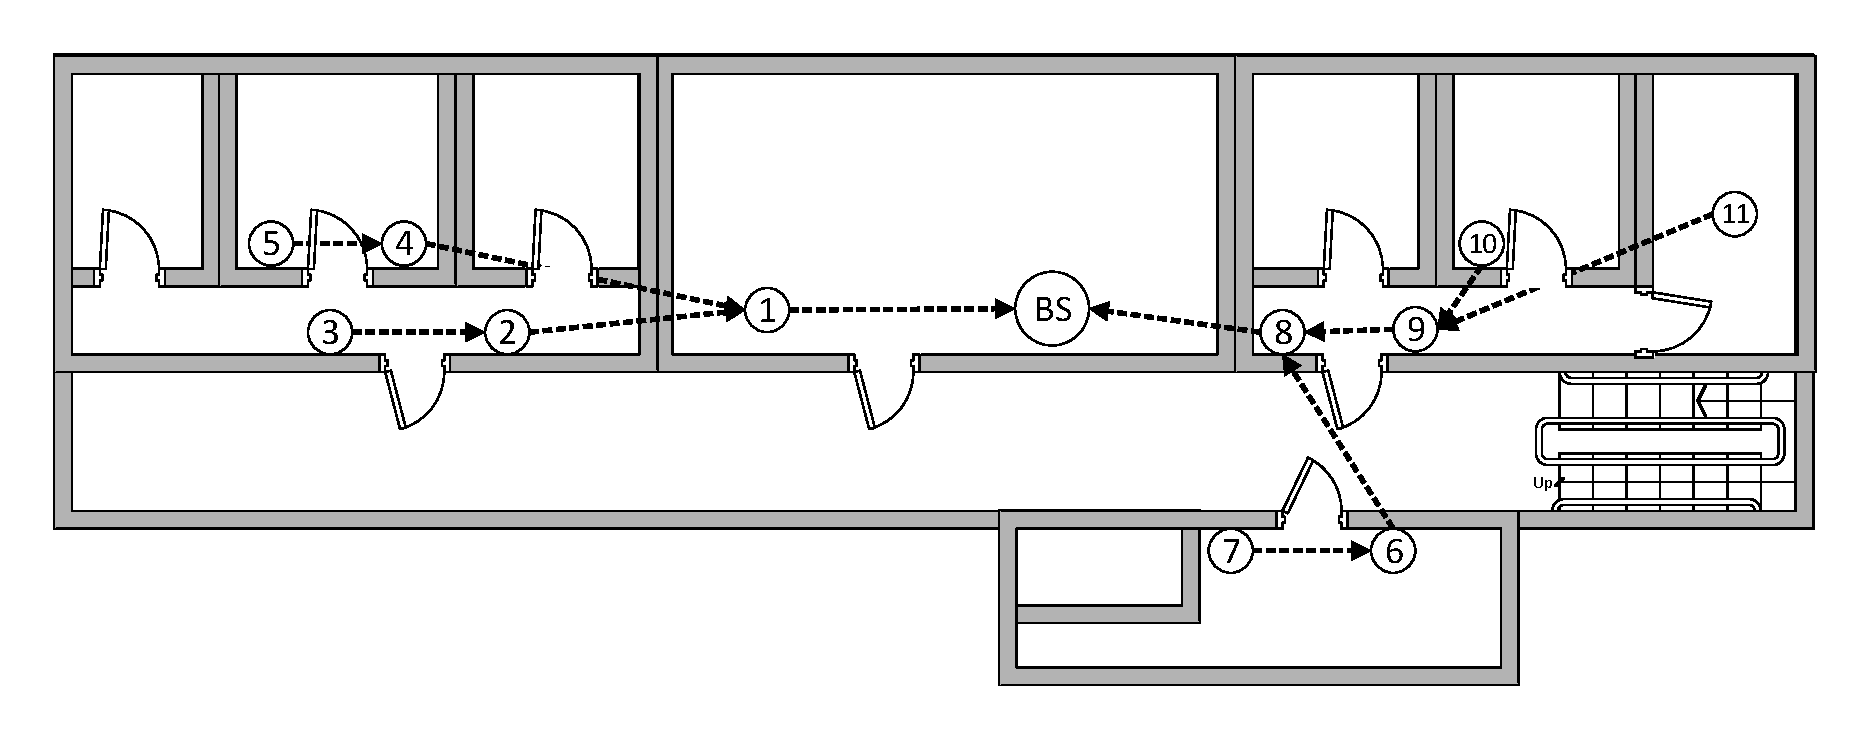
\includegraphics[width=1\linewidth, height=4cm]{floor-plan}
	\vspace{-0.85cm}
	\caption{\textbf{The indoor testbed.}}
	\label{fig:floor-plan}
	\vspace{-0.35cm}
\end{figure}

\subsection{Experimental Evaluation} \label{sec:evaluation}

We have evaluated the detection performance of our RADIUS implementation in an indoor testbed (Figure \ref{fig:floor-plan}) consisting of 12 TelosB motes, deployed in several offices of a university building. Each sensor node runs an application that collects environmental data and sends it to the sink every 2 seconds following a tree-based routing topology. We instrumented a Detection Agent on each sensor node and ran the VCC on a PC connected to the sink node (Base Station).


To configure the RADIUS system, we adopt the system parameter settings suggested in the previous analysis (Section \ref{sec:parameterChoice}). Table \ref{tab:parameter} summarizes the suggested parameter settings. After a training period of about 5 minutes, RADIUS starts the detection phase for a period of about 24 hours. During the experiment, we logged the received alarms, the RSSI traces and the PDR traces. Figure \ref{fig:EVA-1node} demonstrates our results of detecting link quality anomalies on one of the links.

\begin{table}[t]
	\centering
	%\vspace{-0.3cm}
	\caption{\textbf{The system parameter settings used in the evaluation.}}
	\vspace{-0.3cm}
        \footnotesize
	\begin{tabulary}{0.95\textwidth}{|l|l|l|}
		\hline
		\textbf{Techniques} & \textbf{Parameters} & \textbf{Settings} \\ 
		\hline
		\textbf{Bayesian} & initial $P(H_g)$ & 0.8\\
		\textbf{Thresholding} & maximum $P(H_g)$ & 0.99\\
		\hline
		\textbf{Training Set Size} & sample number $N_s$ to compute $\sigma_s$ & 250 \\
		\textbf{Estimation} & max. estimated error of mean $E_{\mu} $ & 1 dBm\\
		\hline
		\textbf{Data Smoothing}	& sliding window size $l$ & 3 \\
		\hline
		\textbf{Training Set Update}	& update window size $l_{update}$ & 50 \\ 
		\hline
		\textbf{\textit{A Priori} Probability} & max. alarm number $N_{alarm}$ & 5 \\ 
		%\hline			
		\textbf{Refinement} & adjustment step $\delta$ & 0.003 \\ 
		\hline
	\end{tabulary}
	\vspace{-0.6cm}
	\label{tab:parameter} 
\end{table}
%---------------------- 

\begin{figure}[t]
	\centering
	%\vspace{-0.1cm}
	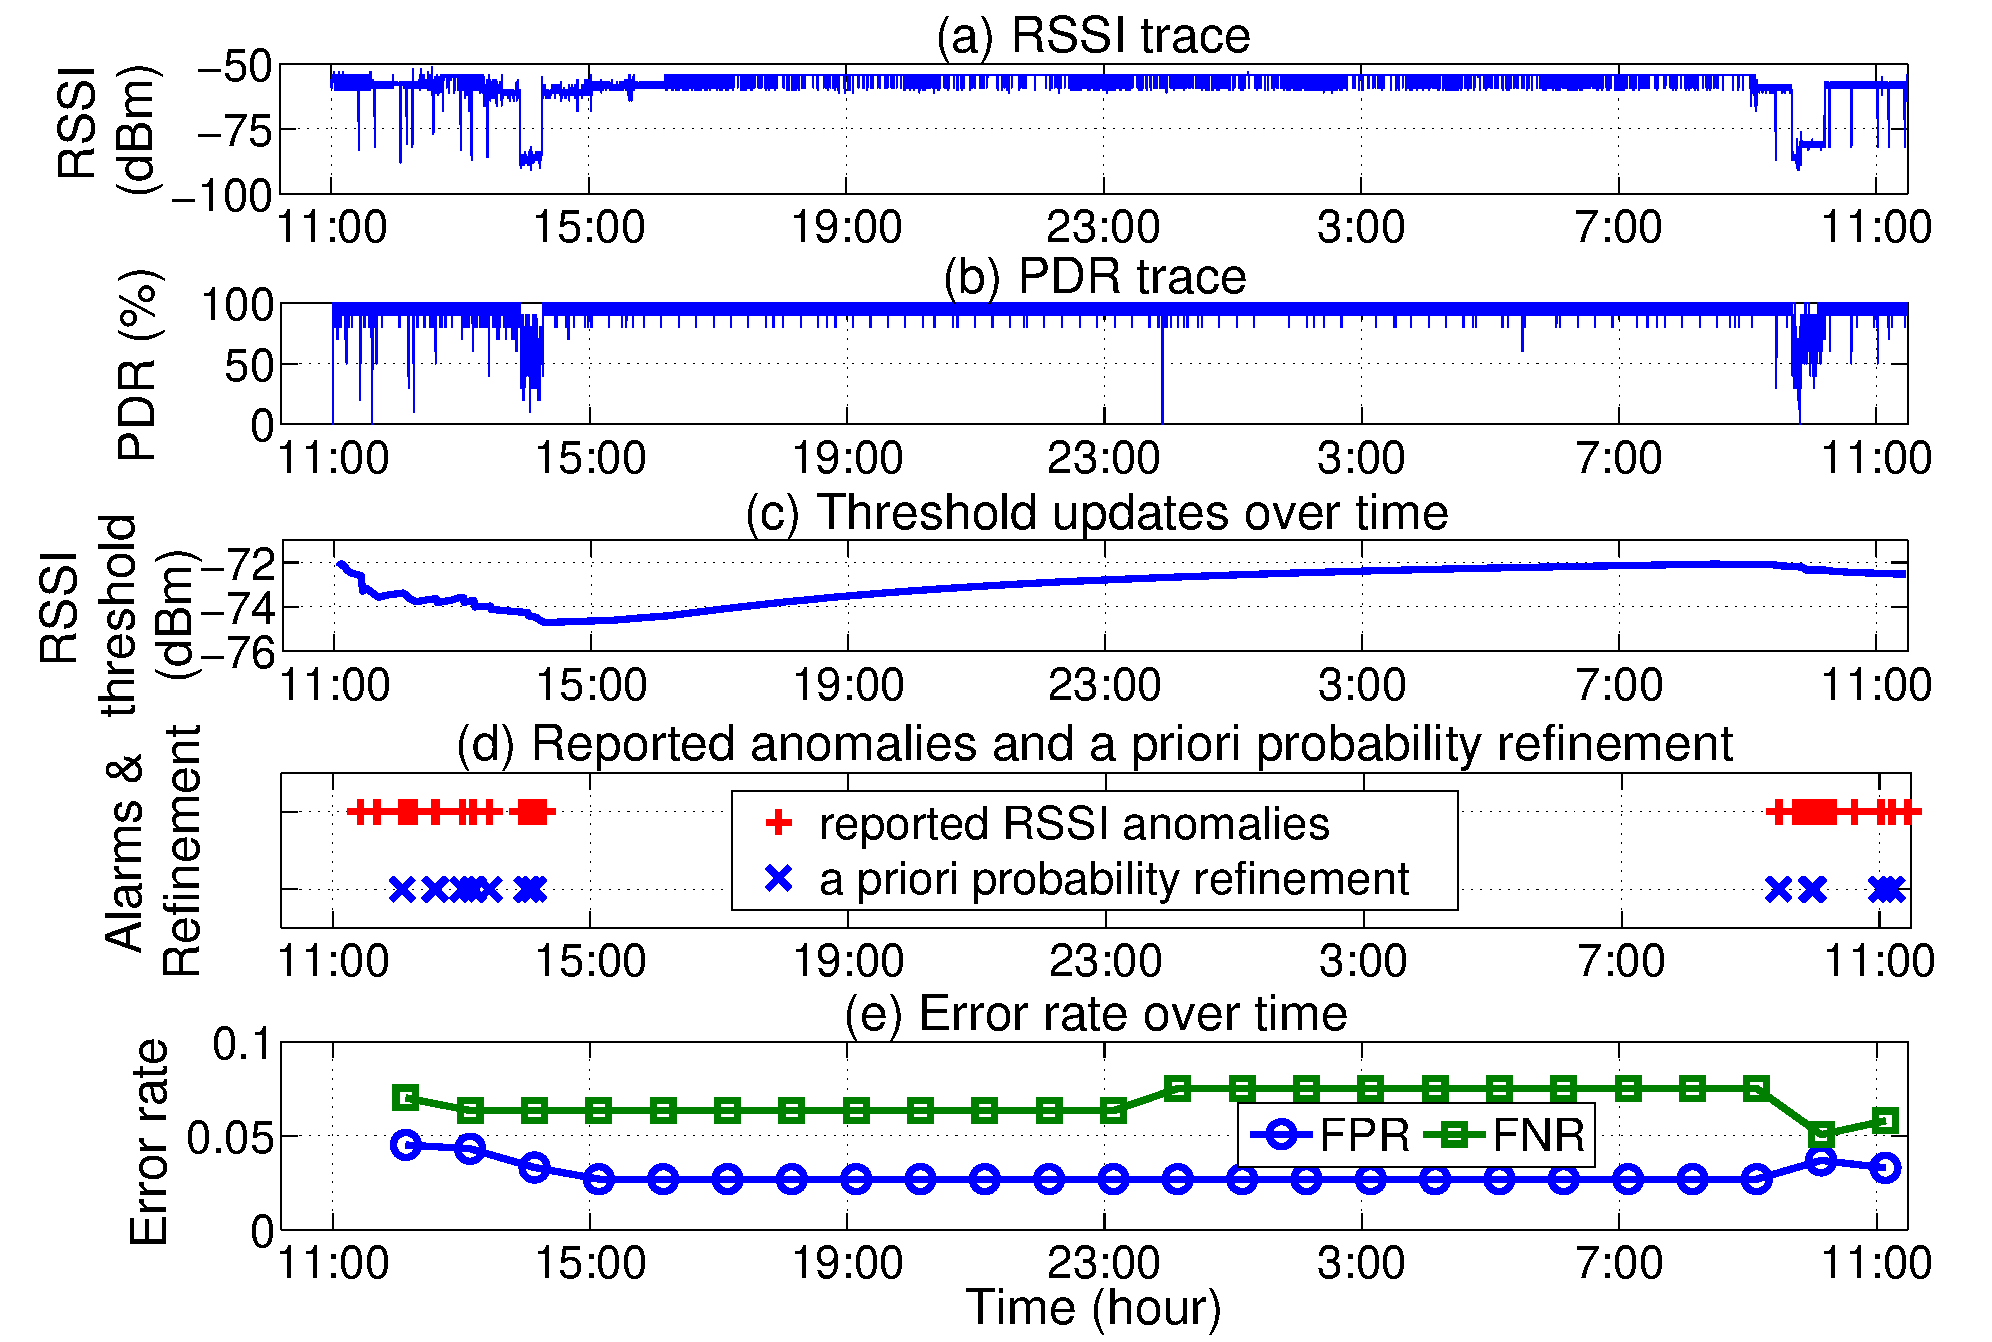
\includegraphics[width=1.0\linewidth, height = 7.5cm]{8-Testbed-1node-24hours}
	\vspace{-0.7cm}
	\caption{\textbf{Experimental results for link quality anomaly detection of the link from node 11 to node 9. The  experiment was run for 24 hours, from 11:00 am till 11:00 am on the next day.}}
	\label{fig:EVA-1node}
	\vspace{-0.2cm}
\end{figure}


From the PDR trace depicted in Figure~\ref{fig:EVA-1node}(b), we can observe that the link frequently experienced high packet losses during the first 4 hours and the last 3 hours due to the bad channel quality caused by the students' movements crossing the communication link (see Figure~\ref{fig:EVA-1node}(a)). The received alarms that reported such anomalous link quality degradation are marked in red in Figure~\ref{fig:EVA-1node}(d). The results show a good detection accuracy. The overall FNR and FPR of detecting the anomalous RSSI degradation for this link over 24 hours are 5.1\% and 4\%, respectively. 

In addition, we can see from Figure~\ref{fig:EVA-1node}(e) that RADIUS can keep the error rate stable over the detection period. Figure~\ref{fig:EVA-1node}(c) clearly shows that the threshold is adaptive to RSSI variations due to the environment changes. From our analysis based on the logged refinement points (marked in Figure~\ref{fig:EVA-1node}(d)), RADIUS refines the \textit{a priori} probability at around 13:00 on the first day and 10:00 on the next day to reduce FPR and thus maintain the detection accuracy. 

To demonstrate that RADIUS can robustly achieve high detection accuracy for all the links across the entire deployed network, we plot in Figure \ref{fig:EVA-11nodes} the error rate for every link in the testbed. The figure shows that with a set of global parameter settings (listed in Table \ref{tab:parameter}), RADIUS achieves a low error rate for every link in the network (6.13\% on average). %This is achieved by the Bayesian thresholding which provides near optimal detection accuracy with the supporting hreshold adaptation techniques. 


%we can see that the system with a set of global parameter settings achieves a low error rate for every node in the network (6.13\% in average). %Note that node 6 has highest FPR and FNR among all nodes. This is because the normal RSSI trace of the link 6 - 8 highly overlaps its abnormal RSSI trace, making the detection more difficult. 

\begin{figure}[t]
	\centering
	%\vspace{-0.1cm}
	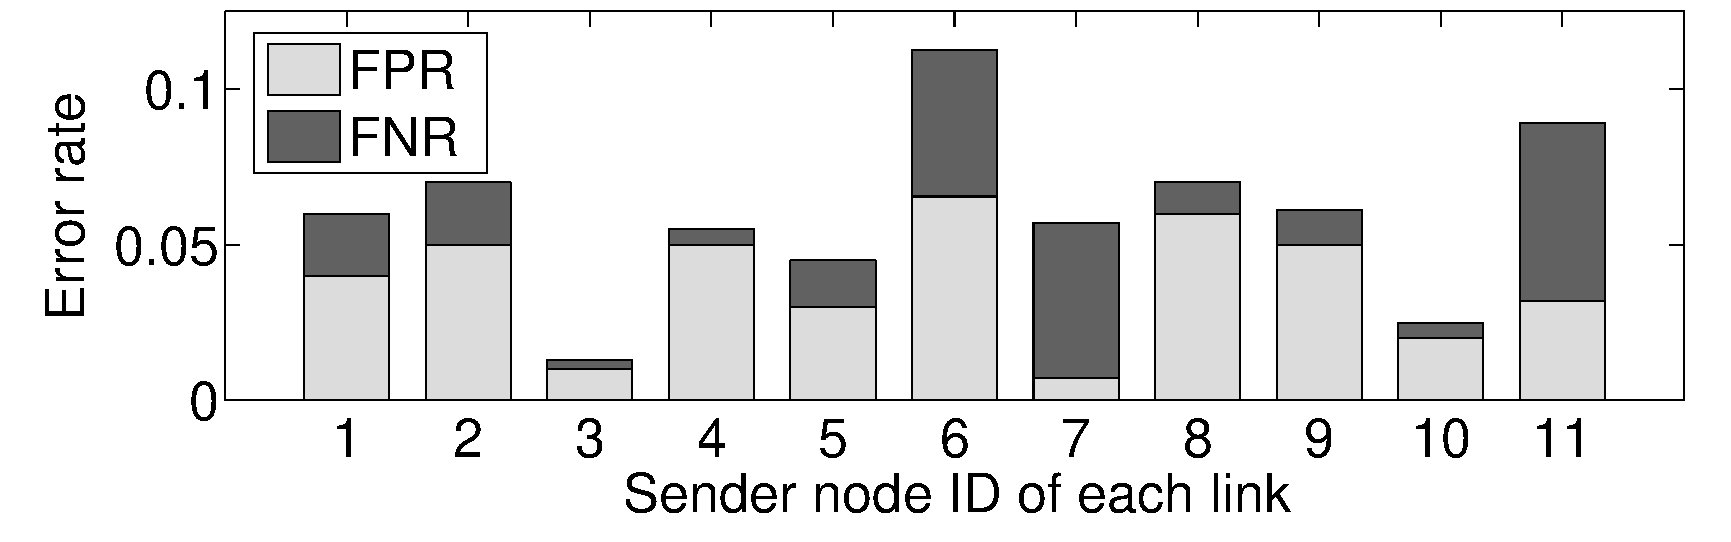
\includegraphics[width=1.0\linewidth]{9-Testbed-12nodes}
	\vspace{-0.7cm}
	\caption{\textbf{The error rates for every link in the network (Figure \ref{fig:floor-plan}).}}
	\label{fig:EVA-11nodes}
	\vspace{-0.55cm}
\end{figure}






